\section{Implementation}
\label{sec:imple}
To invert such a complex system (figure \ref{fig:plane_model}), two layers of inversion are proposed by \cite{hector}, namely for the fast and slow dynamics. Directly controlling these are three of the four actuator control inputs, the control surfaces for the aileron, elevon and rudder. These will therefore be the output of the nonlinear inversion control. 

\subsection{Fast Dynamics}
To invert the fast dynamics equation \ref{eq:fast_dynamics} must be differentiated once, to account for both the actuator dynamics in equation \ref{eq:actuator_dynamics} and the wind effects. Doing so yields the jerk vector given by, as per \cite{hector}

\begin{equation}
\begin{split}
\begin{bmatrix}
\ddot{p}\\
\ddot{q}\\
\ddot{r}
\end{bmatrix}
= \dfrac{1}{2}\rho SI^{-1} \left\lbrace V_a^2 C_\delta \xi^{-1}
\begin{bmatrix}
\delta^d_{ail}-\delta_{ail}\\
\delta^d_{ele}-\delta_{ele}\\
\delta^d_{rud}-\delta_{rud}
\end{bmatrix}
+V_a^2C_c\dot{R_a}+\right.\\
\left. 2V_a\dot{V_a}\left(
\begin{bmatrix}
bC_l\\
\bar{c}C_m\\
bC_n
\end{bmatrix}
+ C_\delta 
\begin{bmatrix}
\delta_{ail}\\
\delta_{ele}\\
\delta_{rud}
\end{bmatrix}
\right) \right \rbrace + I^{-1}\left(\dfrac{1}{4}\rho SV_aC_k-I_n\right)\dot{\Omega}
\label{eq:jerk}
\end{split}
\end{equation}

where

\begin{gather*}
I=
\begin{bmatrix}
I_{xx} & 0 & -I_{xz}\\
0 & I_{yy} & 0\\
-I_{zx} & 0 & I_{zz}
\end{bmatrix}\\
I_n=
\left[\begin{smallmatrix}
-I_{xz}q & (I_{zz}-I_{yy})r-I_{xz}p & (I_{zz}-I_{yy})q\\
(I_{xx}-I_{zz})r+2I_{xz}p & 0 & (I_{xx}-I_{zz})p-2I_{xz}r\\
(I_{yy}-I_{xx})q & (I_{yy}-I_{xx})p+I_{xz}r & I_{xz}q
\end{smallmatrix}\right]\\
\xi=
\begin{bmatrix}
\xi_{ail} & 0 & 0\\
0 & \xi_{ele} & 0\\
0 & 0 & \xi_{rud}
\end{bmatrix}\\
C_c=
\begin{bmatrix}
0 & bC_{l_\beta} & -\dfrac{b^2}{2V_a^2}(C_{l_p}p+C_{l_r}r)\\
\bar{c}C_{m_\alpha} & 0 & -\dfrac{\bar{c}^2}{2V_a^2}C_{m_q}q\\
0 & bC_{n_\beta} & -\dfrac{b^2}{2V_a^2}(C_{n_p}p+C_{n_r}r)
\end{bmatrix}\\
C_k=
\begin{bmatrix}
b^2C_{l_p} & 0 & b^2C_{l_r}\\
0 & \bar{c}^2C_{m_q} & 0\\
b^2C_{n_p} & 0 & b^2C_{n_r}
\end{bmatrix}\\
\dot{Ra} =  [\dot{\alpha} \quad \dot{\beta} \quad \dot{V_a}]^T
\end{gather*}

To do a feedback linearisation, a pseudo input must be chosen, in this case $\tau = \ddot{\Omega}$. The feedback control law will therefore be, solving equation \ref{eq:jerk} for $\delta^d$,

\begin{equation}
\begin{split}
\begin{bmatrix}
\delta^d_{ail}\\
\delta^d_{ele}\\
\delta^d_{rud}
\end{bmatrix}
=\dfrac{1}{V_a^2}\xi C_\delta^{-1}\left\lbrace\dfrac{2I}{\rho S}\tau - \dfrac{2}{\rho S}(\dfrac{1}{4}\rho S V_aC_k - I_n)\dot{\Omega}\right.\\
\left. -2V_a\dot{V_a} \left(
\begin{bmatrix}
bC_l\\
\bar{c}C_m\\
bC_n
\end{bmatrix}
+ C_\delta \delta\right)-V_a^2C_c\dot{R_a} \right\rbrace+ \delta
\label{eq:control_law}
\end{split}
\end{equation}


Indeed, by replacing the equation from equation \ref{eq:control_law} in the jerk equation \ref{eq:jerk}, the equation $\ddot{\Omega} = \tau$ is obtained, resulting in a successfully inverted system.


The wind effects will appear in the terms including $\dot{R}_a =  [\dot{\alpha} \quad \dot{\beta} \quad \dot{V_a}]^T$, as the equation defining $\dot{V_a}$ can be obtained differentiating the norm of the speed relative to the ground. The value of $\dot{R}_a$ can be computed from equation \ref{eq:alphabetadot}.

Should all of the parameters mentioned in the equations above be known and no inversion error be made, the resulting system $\ddot{\Omega}=\tau$ will be both linear and decoupled, having three pseudo inputs $\tau = [\tau_p \quad \tau_q \quad \tau_r]^T$. As mentioned in the previous section, the next step of the nonlinear inversion shall be to propose a linear controller for this resulting system. Taking the desired rotation rates $\Omega^d$ as inputs a control law for $\tau$ may be defined, first considering no neural network adaptation
\begin{equation}
\tau = -K_P (\Omega-\Omega^d)-K_D (\dot{\Omega}-\dot{\Omega}^d)+\ddot{\Omega}^d
\label{eq:linear_controller}
\end{equation}
Where $K_P$ and $K_D$ are chosen to ensure stability and reference tracking. The previous equation can also be written as
\begin{equation}
\ddot{e}=-K_P e - K_D \dot{e}
\end{equation}
assuming that an ideal inversion is obtained and $\tau=\ddot{\Omega}$, and introducing an error variable $e=\Omega-\Omega^d$. 

This way the initial non-linear system becomes a second order linear one, for which natural frequencies and damping values for each dimension must be chosen. Choosing $x_1=e_i$ and $x_2=\dot{x_1}$ for a given dimension $i$ of $\Omega$, either $p,q,r$. Then comes the state equation
\begin{equation}
\begin{bmatrix}
\dot{x_1}\\
\dot{x_2}
\end{bmatrix}=
\begin{bmatrix}
0 & 1\\
-K_{P_i} & -K_{D_i}
\end{bmatrix}
\begin{bmatrix}
x_1\\
x_2
\end{bmatrix}
\end{equation}

The characteristic equation is then obtained as 

\begin{equation}
\begin{split}
\text{det}(\lambda I-A_i)= \lambda^2 + 2\lambda\zeta_i \omega_{n_i} +  \omega_{n_i}^2\\ = \lambda^2 + \lambda K_{D_i} + K_{P_i} = 0
\end{split}
\end{equation}
\begin{gather}
\zeta_i = \dfrac{K_{D_i}\sqrt{K_{P_i}}}{2K_{P_i}}\\
\omega_{n_i}=\sqrt{K_{P_i}}
\end{gather}

The chosen values are given in table \ref{tab:tau_dynamics}.

\begin{table}[htbp]
  \centering
  \caption[Linearised system chosen dynamics]{Linearised system chosen dynamics}
    \begin{tabular}{rcccc}
    \toprule
    $i$   & $K_{P_i}$ & $K_{D_i}$ & $\zeta_i$ & $\omega_{n_i}$(rad $s^{-1}$) \\
    \midrule
    $p$   & 100   & 20    & 1     & 10 \\
    $q$   & 5     & 1     & 0.22 & 2.24 \\
    $r$   & 100   & 20    & 1     & 10 \\
    \bottomrule
    \end{tabular}%
  \label{tab:tau_dynamics}%
\end{table}%


From this point the next step will be to obtain the desired values of $\Omega$. These are obtained using another PD controller, using Euler angles values to control rotation rates. The yaw rate was set to zero as the feedback linearisation decouples the plane movement, using roll and pitch motion to turn the aircraft.

\begin{subequations}
\begin{equation}
p= k_{P_p} (\phi^d-\phi) + k_{D_p} (\dot{\phi^d}-\dot{\phi})
\end{equation}
\begin{equation}
q= k_{P_q} (\theta^d-\theta) + k_{D_q} (\dot{\theta^d}-\dot{\theta})
\end{equation}
\begin{equation}
r=0
\end{equation}
\label{eq:omega_PD}
\end{subequations}

\subsection{Slow Dynamics}

It is now possible to control the attitude of the aircraft, and the fast control loop design is completed. To follow 4D trajectories however, a guidance control loop must be designed to feed attitude and thrust reference values to the system described so far and to achieve the goal of position tracking over time. First the dynamics for speed ($V_a$), heading ($\psi$) and flight path angle ($\gamma = \theta - \alpha$), neglecting wind disturbances, from Newton's Law in the wind frame, are given by
\begin{subequations}
\begin{equation}
\dot{V_a} = \dfrac{1}{m}(T\cos \alpha -D - mg\sin \gamma)
\label{eq:va_dot}
\end{equation}
\begin{equation}
\dot{\gamma} = \dfrac{1}{mV_a}(T\sin \alpha +L - mg\cos \gamma)
\label{eq:gamma_dot}
\end{equation}
For the yaw rate it comes that 

\begin{equation}
\dot{\psi} = \dfrac{g}{V_a} \tan \phi
\label{eq:psi_dot}
\end{equation}
\end{subequations}


After choosing the desired dynamics to control these variables, the equations above must be solved for both the thrust reference $T$, the desired AoA and $\psi$. From these last two, knowing the current pitch angle $\theta$, the input for the fast dynamics controller is obtained. The desired dynamics were chosen as first order systems as
\begin{subequations}
\begin{equation}
\dot{V_a} = \dfrac{1}{\xi_{V_a}}(V_a^d-V_a)
\label{eq:va_dot_des}
\end{equation}
\begin{equation}
\dot{\gamma} = \dfrac{1}{\xi_{\gamma}}(\gamma^d-\gamma)
\label{eq:gamma_dot_des}
\end{equation}
\begin{equation}
\dot{\psi} = \dfrac{1}{\xi_{\psi}}(\psi^d-\psi)
\label{eq:psi_dot_des}
\end{equation}
\end{subequations}

%%%%%%%%%%%%%%%%%%%%%%%%%%%%%%%%%%%%%%%%%%%%%%%%%%%%%%%%%%%%%%%%%%%%%%
\subsection{Online Neural Network}

From an error-less nonlinear inversion, the pseuso-input $\tau$ would directly control $\ddot{\Omega}$ as it was seen previously. However, in case of inversion errors, that can be caused by several factors such as modelling errors or external disturbances, comes that $\tau = \ddot{\Omega}^d + \Delta$, where $\Delta = \ddot{\Omega}- \ddot{\Omega} ^d$. 

This method adds an adaptive component $\tau_{NN}$ to the pseudo input that will approximate the behaviour of the $\Delta$ error. The resulting control law will be given by 
\begin{equation}
\tau + \tau_{NN} = \ddot{\Omega}^d + \Delta
\end{equation}
For which as $t \rightarrow \infty$, $\tau_{NN} \rightarrow \Delta$, thus adaptively minimizing inversion errors. To do so a simple neural network architecture was chosen: a network with a single hidden layer with therefore two sets of weights $V$ and $W$ that will need to be trained, corresponding to the input weights and the hidden layer ones. As for the activation functions for the hidden layer a sigmoid function was chosen, $sig(x)=\dfrac{1}{(1+e^{-x})}$. As the outputs do not need to be bound between $[0;1]$, the chosen output function was a linear one. Indeed sigmoid output functions are usually used in applications where the output must be a boolean value.

There are quite some challenges in designing a feed forward neural network. Besides choosing the number of layers and neurons per layer, the inputs of the network must also be chosen carefully. Some rules to choose the correct inputs are given by \cite{NN_inputs}:
\begin{itemize}
\item \textbf{Relevance}: This is the most important consideration to have while choosing a set of inputs, this set must be sufficiently informative of the state of the system for the network to perform correctly. A NN will perform poorly if the output behaviour is not correlated to its input.
\item \textbf{Redundancy}: A large value of redundant and irrelevant input variables will not only increase the needed computational effort of the NN, but will also increase the difficulty to train the weights of the network and add noise to the system.
\end{itemize}

Another consideration about the chosen inputs that must also be taken into account is their range. The sigmoid function $sig(x)$ used reaches around 73\% when $x=1$ and 88\% when $x=2$. For some cases the inputs might therefore need to be normalized. While this is quite a trivial task in the case of batch training, as the minimum and maximum value of each input is easily obtained before even starting training, such is not the case for online training, and a maximum and minimum value must be proposed \emph{a priori} for each input. The average of these values should also be close to zero. Should the input not be normalized and reach absolute values much greater than the unity, its activation function output would be constant and the system would therefore not react to input change. This, clearly, is not desirable. To map the input $x$ knowing its minimum and maximum values to its normalized equivalent $y$, the following equation is used

\begin{equation}
y=2\dfrac{x-x_{min}}{x_{max}-x_{min}}-1
\label{eq:normalisation}
\end{equation}

For this  particular case, the state variables of the fast dynamics where used as inputs of the network, namely $\Omega$ and $\dot{\Omega}$.

A backpropagation algorithm was used to train both sets of weights online. This algorithm, however, must have an error function that will be minimized by iteratively changing the values of the weights $V$ and $W$. As seen previously, an inversion error $\Delta$ will be present, where $\tau = \ddot{\Omega}^d + \Delta$. This error must be computed for each iteration to train the network to approximate this error. The error can be expressed as $\Delta=\tau - \ddot{\Omega}^d$.
From the control law used to obtain $\tau$ (\ref{eq:linear_controller}) it comes that
\begin{equation}
\Delta = -K_P(\Omega-\Omega^d)-K_D(\dot{\Omega}-\dot{\Omega}^d)
\label{eq:inversion_error}
\end{equation}
Finally the cost function used to train the network is given by

\begin{equation}
J=\dfrac{1}{2}(\Delta-y_{NN})^2
\label{eq:NN_cost}
\end{equation}

From this cost function, the weights can be updated iteratively, where the variation of a given weight from the $i^{th}$ input of the $j^{th}$ neuron from a layer $w$ is given by

\begin{equation}\label{eq:update_law}
\Delta w_{ij} = - \alpha \frac{\partial J}{\partial w_{ij}}
\end{equation}

Where $\alpha$ is the learning coefficient. The chain rule can be used to compute $\frac{\partial J}{\partial w_{ij}}$ as such

\begin{equation}\label{eq:gradient}
\frac{\partial J}{\partial w_{ij}} = \frac{\partial J}{\partial sig(sum_j)}\frac{\partial sig(sum_j)}{\partial sum_j}\frac{\partial sum_j}{\partial w_{ij}}
\end{equation}

Where $sum_j$ is given by

\begin{equation}\label{eq:def_sum}
sum_j = \sum ^n_{k=1} w_{kj} x_k
\end{equation}

Where $x_k$ is the output of the $k^{th}$ neuron of the previous layer (or of the $k^{th}$ input in the case of the first weight layer).

These three factors of equation \ref{eq:gradient} can now be easily computed. The last two factors are independent of weather $x_j$ is a hidden or output layer and will for this reason be calculated firstly. 

For an output layer, where values may be unbounded, linear output functions may be used, for which $\frac{\partial f(sum_j)}{\partial sum_j}$ has a trivial solution. For the case of a logistic sigmoid activation function it comes that 

\begin{equation}
\frac{\partial f(sum_j)}{\partial sum_j}=f(sum_j)(1-f(sum_j))
\end{equation}

For the term $\frac{\partial sum_j}{\partial w_{ij}}$, from \ref{eq:def_sum} this partial derivative is easily computed

\begin{equation}
\frac{\partial sum_j}{\partial w_{ij}} = \frac{\partial \left(\sum ^n_{k=1} w_{kj} x_k\right)}{\partial w_{ij}} = x_i
\end{equation}

For the output layer, the first term of equation \ref{eq:gradient} can easily be evaluated, as $x_j=y$ for such a case, giving

\begin{equation}
\frac{\partial J}{\partial x_j}=\frac{\partial (\frac{1}{2} (\Delta-y_{NN})^2)}{\partial y_{NN}}= \Delta-y_{NN}
\end{equation}

For input layers however, this derivative is less obvious to estimate. One can consider that the error function $J$ is a function of the inputs of all neurons that take $x_j$ as input. Let $S$ be such a set of inputs, from the total derivative to $x_j$ it comes that

\begin{gather}
\frac{\partial J}{\partial x_j} = \sum _{s\in S}\left( \frac{\partial J}{\partial x_s}\frac{\partial x_s}{\partial sum_s}\frac{\partial sum_s}{\partial x_j}\right)=\\
\sum _{s\in S}\left( \frac{\partial J}{\partial x_s}\frac{\partial f(sum_s)}{\partial sum_s}w_{js}\right)
\end{gather}

Note that the term $ \frac{\partial J}{\partial x_s} $ represents the all the derivatives of the errors with respect to the outputs of the next layer of neurons. Once this derivative is computed the new set of weights for both layers can be estimated from the update law \ref{eq:update_law}.


\subsection{Guidance Law}

The final step of the controller design will be to propose a guidance law to obtain the values of $V_a^d$, $\gamma^d$ and $\psi^d$ from the X,Y and Z reference values along time. For these laws it was assumed that the position reference was given relative to a frame of reference with the origin on the Earth surface, with the $Z$ axis pointing upwards. The guidance controller therefore implements the following equations, assuming the errors $\delta x = x_r - x$, $\delta y = y_r - y$ and $\delta z = z_r-z$.

\begin{subequations}
	\begin{gather}
	\delta V_a = \dfrac{1}{\tau_{V_a}}(\sqrt{\delta x^2 + \delta y^2 + \delta z^2})\\
	V_a^d= \delta V_a  + V_{a_0}
	\end{gather}
	\begin{equation}
	\psi^d = atan2(\delta y,\delta x)
	\end{equation}
	\begin{equation}
	\gamma^d = \dfrac{1}{\tau_Z}\delta z
	\end{equation}
	\label{eq:guidance_law}
\end{subequations}

This guidance law is intended to be used having at each time interval a $x_r$, $y_r$ and $z_r$ position of a desired trajectory. From these an airspeed, heading and flight path angle must be computed and fed to the controller.

Taking first the airspeed equation from \ref{eq:guidance_law}, $V_{a_0}$ is the desired speed of the aircraft in cruise conditions when following the trajectory. This speed is then corrected by the term $\delta V_a$, increasing or decreasing aircraft airspeed depending on its position relative to the trajectory desired position at a given time, i.e the distance error. By dividing this error by $\tau_{V_a}$, a desired convergence time, the speed correction to the initial value $V_{a_0}$ necessary to follow a 4D trajectory is obtained. Also, from the $x$ and $y$ position errors between the aircraft and the current trajectory waypoint the desired heading can also be computed using the $atan2$ function. Finally, the method used to obtain the Flight Path Angle relies on the error between the height of the aircraft and the desired one to compute it. 

Finally, this control architecture is illustrated by the block diagram of Figure \ref{fig:full_controller}, specifying fast dynamics inversion, the slow dynamics controller and the guidance control law, as well as the online neural network use to improve the controller and adapt to inversion errors and system failures.
\begin{figure*}[h]  
  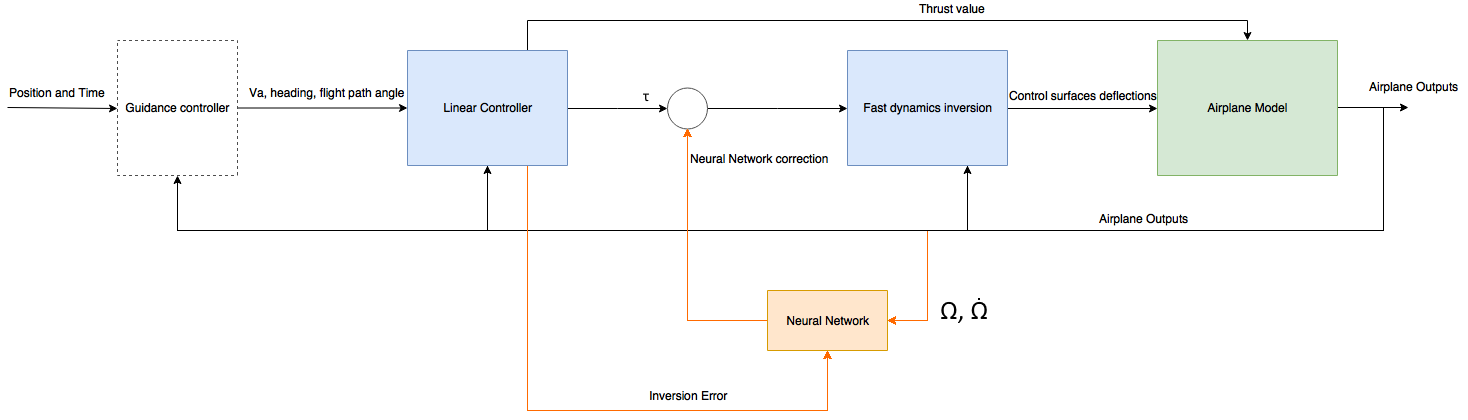
\includegraphics[width=1.05\textwidth]{../Figures/full_controller_special.png}
  \caption[Diagram of the controller architecture]{Diagram of the full controller architecture. In orange is specified the neural network correction system of the initial controller}
  \label{fig:full_controller}
\end{figure*}